\section{Vzorkování z latentního prostoru}
Ve chvíli, kdy je latentní prostor naučeného modelu variačního autoenkodéru uspokojivě zformován, lze přejít k vzorkováni, resp. generování nových MNIST číslic.
\autoref{fig:vae_model_latent_space_sampling} zachycuje vzorkování náhodně vygenerovaných bodů z latentního prostoru naučeného modelu.

\begin{figure}[H]
    \centering
    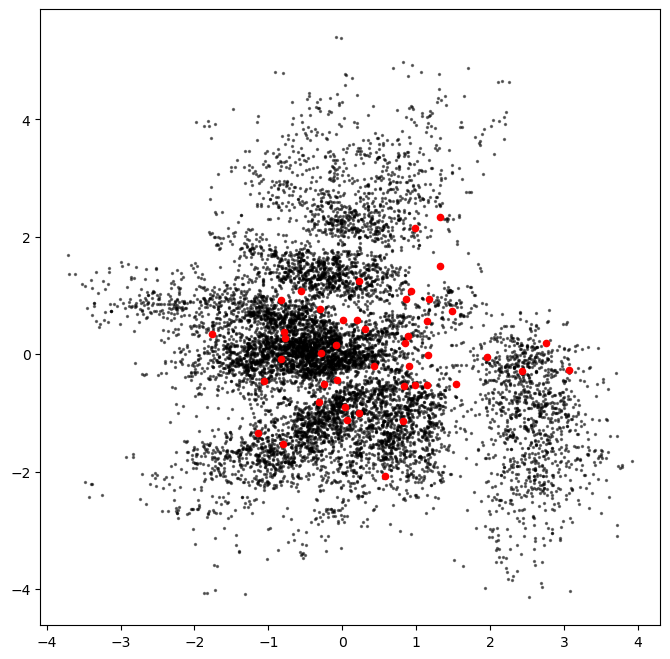
\includegraphics[width=0.95\textwidth]{figures/vae_model_latent_space_sampling.png}
    \caption{Vzorkování z latentního prostoru naučeného modelu. Červené body značí bod z latentního prostoru, který byl použit jako vstup pro dekodér modul. Barevná mapa latentního prostoru, který zachycuje \autoref{fig:vae_model_latent_space}, byla převedena do černé za účelem zřetelné identifikace vzorkovaných bodů.}
    \label{fig:vae_model_latent_space_sampling}
\end{figure}


Výsledné číslice vygenerované dekodér modulem na základě výše uvedených vzorků z latentního prostoru prezentuje \autoref{fig:vae_sampling_results}.
Lze si povšimnout, že většina vygenerovaných číslic \textbf{není deformovaná}.
To je důsledek \textbf{lokální spojitosti latentního prostoru} (v kontrastu s prostým autoenkodérem, jehož latentní prostor je nespojitý).

\begin{figure}[H]
    \centering
    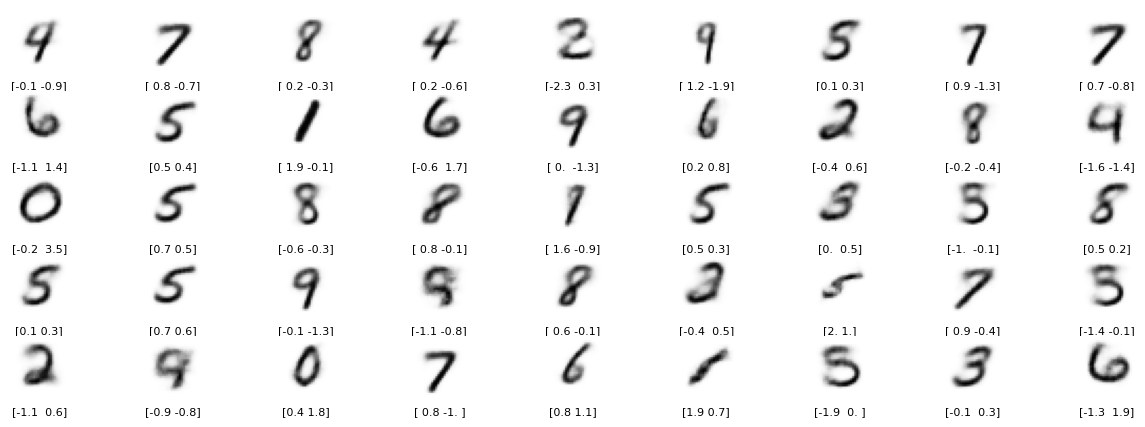
\includegraphics[width=\textwidth]{figures/vae_model_latent_space_sampling_results.png}
    \caption{Vzorky vygenerované naučeným modelem variačního autoenkodéru.}
    \label{fig:vae_sampling_results}
\end{figure}


\autoref{fig:vae_model_latent_space_sampling} a \autoref{fig:vae_sampling_results} názorně znázorňují rovněž aritmetiku latentního prostoru a s ní spojený sémantický význam jednotlivých uskupení.
Například s měnící se hodnotou osy y lze pozorovat změnu sklonu číslice $7$ a její postupný přechod v číslici $9$. Obdobně přechod mezi číslicí $9$ a $4$.
Tyto vztahy jsou určené vypozorovanými charakteristikami a podobnostmi jednotlivých číslic modelem variačního autoenkodéru.
Pro ještě lepší ilustraci aritmetiky v latentním prostoru naučeného modelu variačního autoenkodéru, byly vzorky z náhodné části jeho latentního prostory postupně vyneseny na 2D manifold, který prezentuje \autoref{app:reconstruction_manfiold}.

Proces generování náhodných vzorků z latentního prostoru modelu, a jejich následného generování zachycuje \autoref{app:vae_model_source_code}.